%cSpell:ignore Erol,Sezgin,fancyhdr, hheadheighti,hheadsepi,hfootheighti,graphicx, hfootskipi, Gavrilita, Mihail, AMOO, totalheight, keepaspectratio,UML's, kata, codewars, OOAD, COFFE,ERLANG,caml, kotlin,haskel, ruby, superclass, 
\documentclass[12pt]{article}
%\usepackage[english]{babel}
%actually it works without this package//// cuz it is in english by default... it might be useful //// but not here
% \usepackage{natbib}
% \usepackage{biblatex}

% \usepackage[backend=biber]{biblatex}

%\usepackage{url}
%idk what for it is here, it is not what it seems to be, fuck it
%%\usepackage[document]{ragged2e} 
%%to justify
% i dont use it anymore
\usepackage[utf8]{inputenc}
%%%\usepackage{amsmath}
%%useless for this report... it's for math stuff
\usepackage{graphicx}
%This package enables the user to the importation of graphics into a .tex file and, apart from the usual sizing and rotational facilities, also enables the user to crop or trim an image as desired (e.g., to get rid of surrounding blank margins). The graphicx package is useful if you need to use only a part of a complete image. 
\graphicspath{{images/}}
%% includes pics inside image folder
\usepackage{parskip}
%%this shit . In the document body, don't use \parskip but a blank line to separate paragraphs.there's normally no need to add manual line breaks (\\) in the text.

\usepackage{vmargin}
%%LaTeX package which introduces paper sizes and provides macros for setting document margins. 
\usepackage{enumerate} 
%enumeration of elements  
\usepackage{caption}
%%this is for figures
\usepackage{float}
%% to position exactly the figure 
\usepackage{fancyhdr}
%%To customize the footer and header in your document first import the package fancyhdr with 
% \addbibresource{lab4.bib}
% \bibliography{my_bibliography.bib} 
\PassOptionsToPackage{hyphens}{url}\usepackage{hyperref}
\hypersetup{
    colorlinks=true,
    linkcolor=blue,
    filecolor=magenta,      
    urlcolor=cyan,
}

\renewcommand{\theenumii}{\arabic{enumii}}
\setmarginsrb{3 cm}{2.5 cm}{3 cm}{2.5 cm}{1 cm}{1.5 cm}{1 cm}{1.5 cm}
%%\setmarginsrb{hleftmargini}{htopmargini}{hrightmargini}{hbottommargini}% {hheadheighti}{hheadsepi}{hfootheighti}{hfootskipi
\title{DB Laboratory 2}								
\author{Sezgin E}							
\makeatletter
%%The \makeatletter command temporarily defines »@« as a normal character to enable changes to internal LaTeX macros outside packages (STY) or classes (CLS).
\let\thetitle\@title
%%\let allows you to copy the content of a command into a new command.
\let\theauthor\@author
%%Thus \let\foo\bar defines \foo to have the value that \bar had at the point of definition.
\makeatother
% With \makeatother this process is reversed and the »@« is set to its original character category (other). The »@« is used to protect the internal LaTeX macros. Hence you should be very careful when using these two commands.
\pagestyle{fancy}
%%After that, the "fancy" style is set by \pagestyle{fancy}
\fancyhf{}
%%The command \fancyhf{} clears the header and footer, otherwise the elements of the default "plain" page style will appear. 
\rhead{\theauthor}
%%Prints the text included inside the braces on the right side of the header. 
\lhead{\thetitle}
%%Prints the text set inside the braces on the left side of the header.
\cfoot{\thepage}
%%\cfoot{Page \thepage}  Prints the word "Page" and next the page number which is automatically set by \thepage on the center of the footer. 
        
\begin{document}
        
        %%%%%%%%%%%%%%%%%%%%%%%%%%%%%%%%%%%%%%%%%%%%%%%%%%%%%%%%%%%%%%%%%%%%
        
        \begin{titlepage}
                \centering
                \vspace*{0.5 cm}
                
\includegraphics[scale = 0.11]{LOGO_UTM.jpg}\\[1.0 cm]	% University Logo
                %% Importing a graphic is done by using the command \includegraphics[key1=...,key2=...,etc.]{filename} Optional parameters—called “keys”—enable the figure to be resized, rotated, cropped, trimmed, etc. These keys and their functions are listed below. 
                %• scale = number — a magnification factor 
                %• width = length — the width to which the figure should be scaled1
                %• height = length — the height to which the figure should be scaled2 
                %• totalheight = length — height plus depth of figure (to be used if figure is rotated) 
                %• keepaspectratio = true/false — maintains the height/width ratio 
                %• angle = number — angle (in degrees) by which the figure is to be rotated counterclockwise 
                %• origin = location3 — the point about which rotation is to occur %• draft = true/false — prevents figure from being imported, but created a named box with the dimensions of the figure (this option is used to speed up processing) 
                %• clip = true/false — excludes whatever is outside the bounding box 
                \textsc{\LARGE Technical University of Moldova}\\[2.0 cm]%%\textsc{example text} will display the example text as small caps. All of the letters will be capitalized/uppercase, but they are going to be similar in size to a lowercase letter.	
                % University Name
                \textsc{\Large 19.05.2018}\\[0.5 cm]		% Course Code

                \rule{\linewidth}{0.2 mm} \\[0.4 cm]
                %%The \rule command in normal use produces a simple black box: \rule[raise]{width}{thickness} This is useful for drawing vertical and horizontal lines.

                { \huge \bfseries \thetitle}\\
                %%Anyway, the \bfseries bold the rest of my document, even though I'm using curly braces.
                \rule{\linewidth}{0.2 mm} \\[1.5 cm]
                
                \begin{minipage}{0.4\textwidth}
                        \begin{flushleft} \large
                                \emph{Submitted To:}\\
                                Maria Cojanu\\
                %%If you want to emphasize a word or some text, use \emph. Don't just make the text italic or bold. If needed, you may change the behavior of \emph whenever you wish in the preamble and the whole document will be adjusted accordingly.
                Asst. Univ.\\
                Computer Science Department\\
                            \end{flushleft}
                            \end{minipage}~
                            \begin{minipage}{0.4\textwidth}
                
                            \begin{flushright} \large
                            \emph{Submitted By :} \\
                            Sezgin Erol\\
                
                Group FAF-161\\
                Semester 1\\
                    \end{flushright}
                
                \end{minipage}\\[2 cm]
                
                \vfill Chisinau 2018\\  
        \end{titlepage}
        
        %%%%%%%%%%%%%%%%%%%%%%%%%%%%%%%%%%%%%%%%%%%%%%%%%%%%%%%%%%%%%%%%%%%%
        \pagebreak
        %\tableofcontents
        \subsection*{ General purpose:}
        \subsubsection*{ Learn about Creating a Database}
        
        \subsection*{Tasks:}
        \begin{itemize}
                \item Create physical data stored in the MyDocuments map by setting an increase of the primary 5MB file with the 100MB increase limit and 20MB initial with the 1000MB increase limit. Bypass secondary files to define a new Filegroap implicit,
                setting the increase of 10 MB of secondary files with the limit of 1000 MB.
                \item Create a database, where the log file is physically placed on the MyDocuments / log map, the name
                log file in the operating system environment must be different from the logical one defined in
                physical scheme. It is important that the database you create is compatible with the MS SQL system
                The 2014 Server is accessible to only one user at a time.
                \item Create the database interlining plan built in load 1. Unused sleeping space
                database files must be removed when it reaches 2000Mb. space
                released must be returned to the operating system. This operation must also be run in
                every Friday at 02:00. The report of the implementation of the plan must be saved in the file
                MyDocuments \ SQlreports. They executed the plan. After execution, verifiers
                the results in the log figure.
                \item Create the plan of database interconnection built in exercise 2. The name of the plan will be: Reconstruction index. "Under this plan, the system must undertake the reconstruction
                indexes only on the base tables (excluding the views) of all the existing schemes
                in the data base in question. The free space on the page must be 10 %. 
                After rebuilding, you must to follow the collection of complete statistics on reconstruction indices. The third step of the
                plan must also be the task of deleting history of Backup-Restore operations
                what happened on SQL Server. The history that is older than 6 weeks must be deleted. This
                the plan must be executed every first Sunday of the month. Create the file
                MyDocument/SQL/reports. The plan execution report must be added to this
                file. They executed the plan. After execution, verify the results in the generated log file
                
                
                \end{itemize}
        \subsection*{Task Realization:}
        In figure 1 we can see the process Creating a Database. 
        
        \begin{figure}[H]
                \centering
                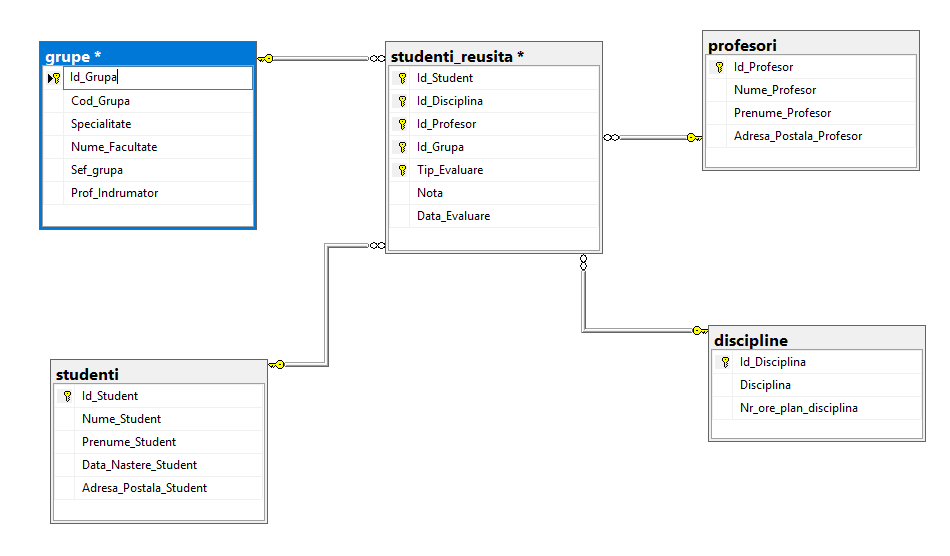
\includegraphics[width=.95\textwidth]{img1.png}
                \caption{ Creating a Database}
        \end{figure}
        \vspace{0.5 cm}
        Here i also set the Filegroups, Initial Sizes , Autogrowth size and the paths
        
        \begin{figure}[H]
                \centering
                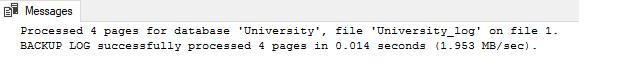
\includegraphics[width=.95\textwidth]{img2.png}
                \caption{Setting  Filegroups }
                I created 2 custom filegroups
        \end{figure}
        \vspace{0.5 cm}

        
        \begin{figure}[H]
                \centering
                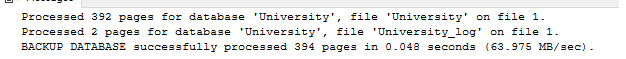
\includegraphics[width=.95\textwidth]{img3.png}
                \caption{Creating Second Database}
        \end{figure}
        \vspace{0.5 cm}

        
        \begin{figure}[H]
                \centering
                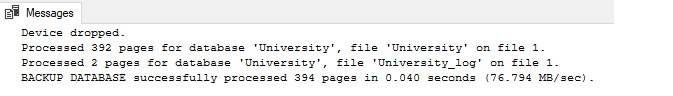
\includegraphics[width=.95\textwidth]{img4.png}
                \caption{Configuring DB Options}
        \end{figure}
        \vspace{0.5 cm}

        I set the single user and SQL Server 2017 compatibility level.        
        \begin{figure}[H]
                \centering
                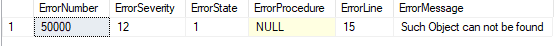
\includegraphics[width=.95\textwidth]{img5.png}
                \caption{Maintenance Plan Wizard}
        \end{figure}
        \vspace{0.5 cm}
        I created a Plan using Wizard and also i set the Schedule.
        Also i selected Shrink Database Option.
        
        \begin{figure}[H]
                \centering
                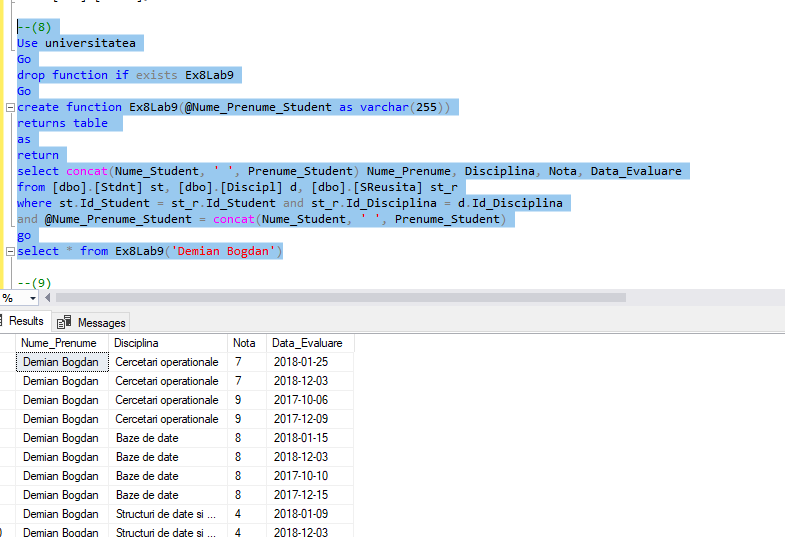
\includegraphics[width=.95\textwidth]{img8.png}
                \caption{Setting folder Location}
        \end{figure}
        \vspace{0.5 cm}

        
        \begin{figure}[H]
                \centering
                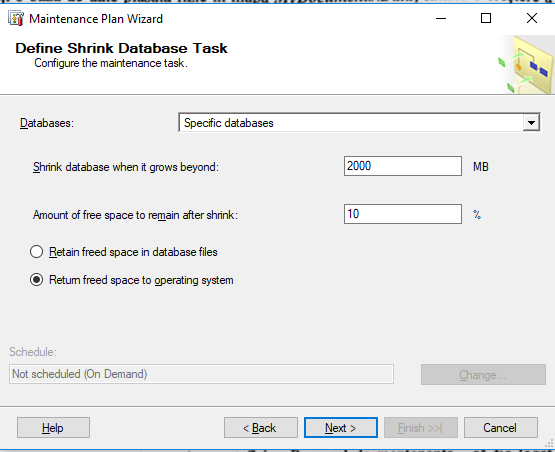
\includegraphics[width=.95\textwidth]{img9.png}
                \caption{Defining Shrink Database Task}
        \end{figure}
        \vspace{0.5 cm}
        I set 2000 MB limit and 10 percent space remaining after shrink
        
        \begin{figure}[H]
                \centering
                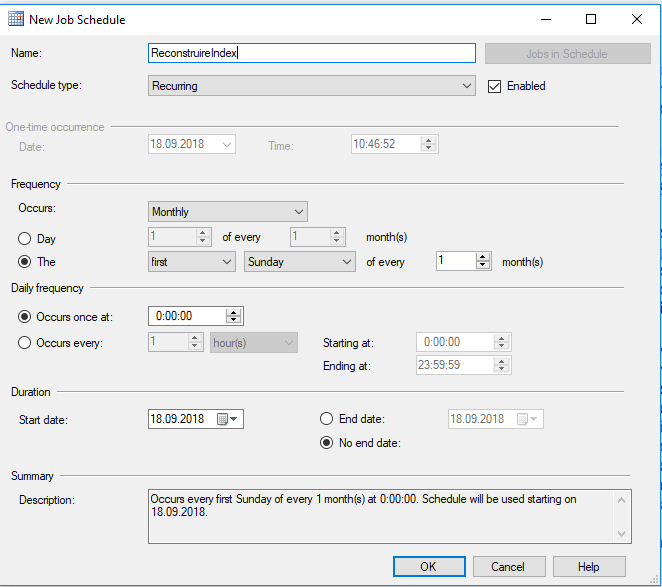
\includegraphics[width=.95\textwidth]{img10.png}
                \caption{The Schedule for 2nd database}
        \end{figure}
        \vspace{0.5 cm}

        
        \begin{figure}[H]
                \centering
                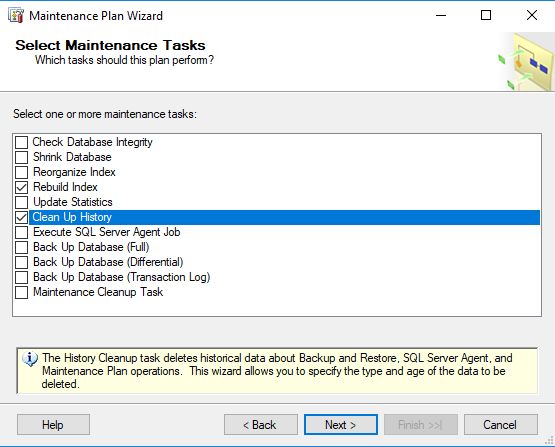
\includegraphics[width=.95\textwidth]{img11.png}
                \caption{Maintenance Tasks for 2nd DB}
        \end{figure}
        \vspace{0.5 cm}

        
        \begin{figure}[H]
                \centering
                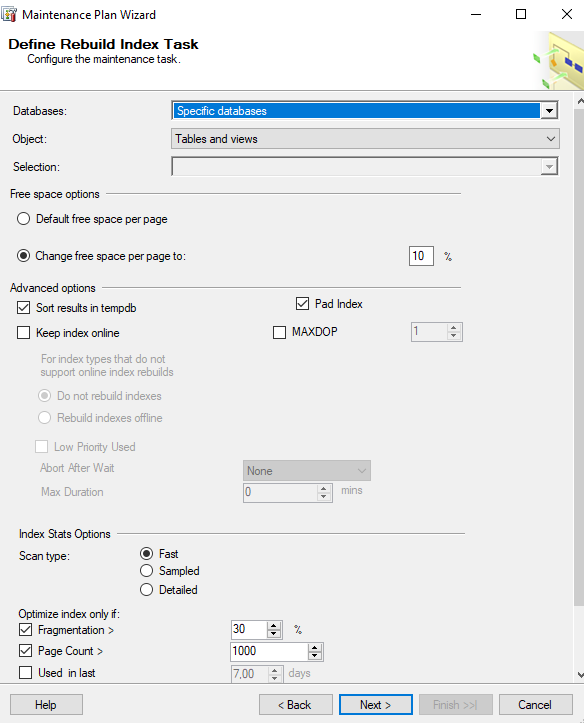
\includegraphics[width=.95\textwidth]{img12.png}
                \caption{Defining rebuild Index}
        \end{figure}
        \vspace{0.5 cm}



        \subsection*{Conclusion}
        During This lab work i find out how to  run SQL server on PC.  And I learned how to configure a Data Base, and to create and set the scheduled plans such a Maintenance. So i Understood that Sql Server Management Studio is Powerful tool to manage Databases.
        \cite{SQLServerManagementStudio}
        

 
\medskip
 
\begin{thebibliography}{9}
\bibitem{SQLServerManagementStudio} 
SQL Server Management Studio, Tutorials for Lab 1 and 2

\end{thebibliography}
                
\end{document}